\documentclass[./blockchain.tex


\begin{document}

    \section{Blockchain}
    \begin{frame}

        \frametitle{Was ist eine Blockchain}

        \begin{itemize}
            \item Erweiterbare Liste von Datenblöcken
            \item Verkettung mittels Konsensverfahren und kryptographischen Methoden
        \end{itemize}

        \begin{figure}[v]
            \centering
            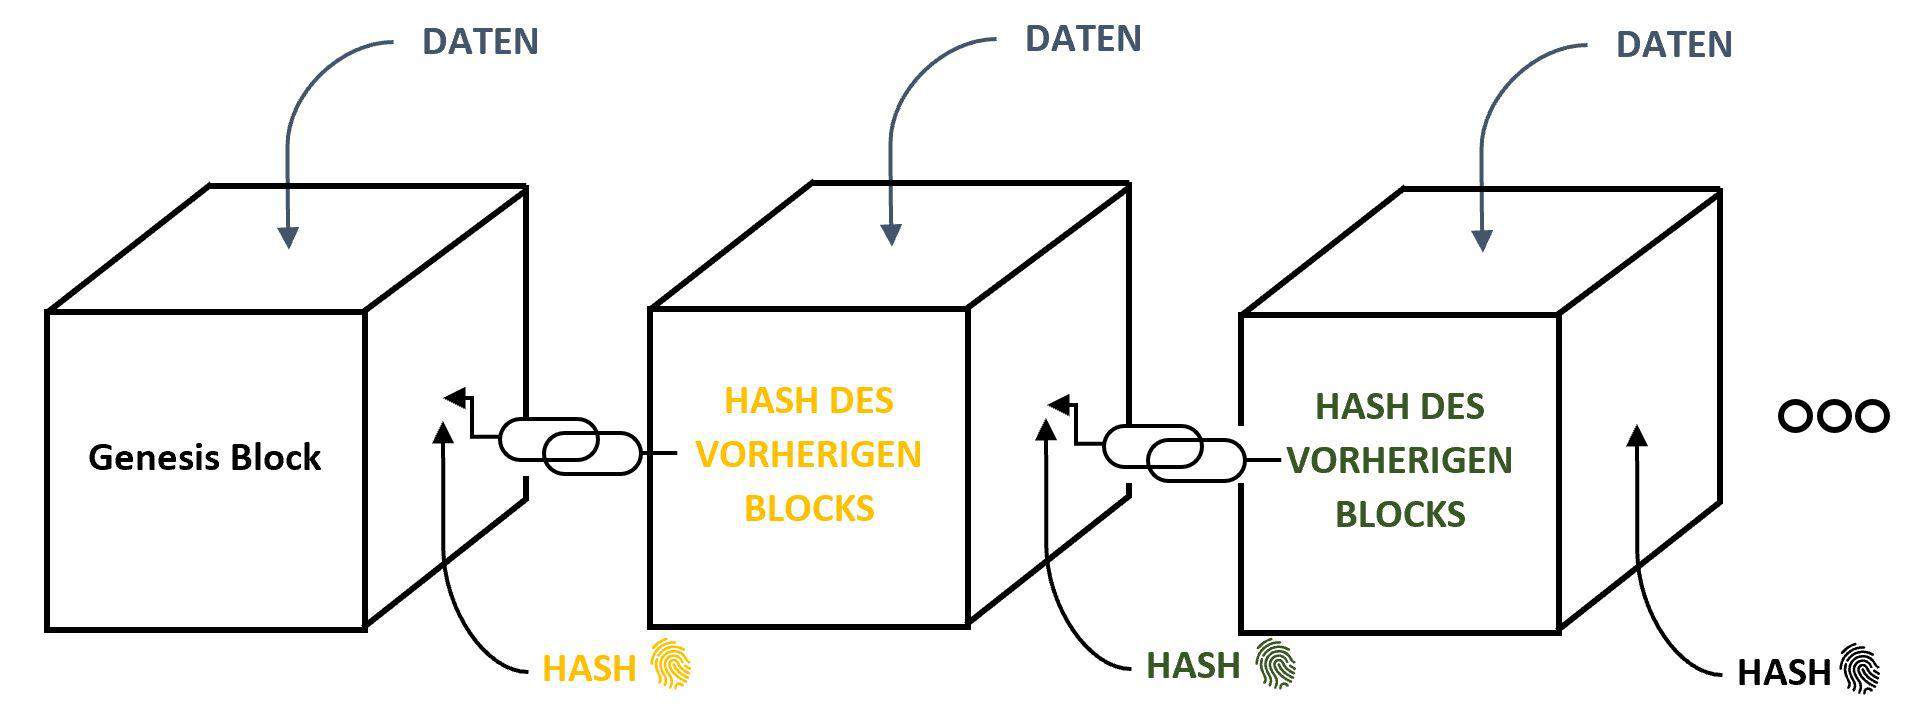
\includegraphics[width=0.8\textwidth]{figures/blockchain}\label{fig:figure}
        \end{figure}

    \end{frame}

    \begin{frame}
        \frametitle{Blockchain als Datenspeicher}

        \begin{itemize}
            \item Daten werde auf hunderten, dezentralen Systemen gleichzeitig gespeichert.
            \item Datenverlust: faktisch nicht möglich.
            \item Daten können nicht gelöscht werden.
            \item Daten können geändert werden - vorherigen Daten bleiben faktisch vorhanden.
            \item Ohne Verschlüsselung sind alle Daten für alle lesbar.
        \end{itemize}

    \end{frame}



    \begin{frame}
        \frametitle{Smart Contracts, Programme und Daten}

        \begin{itemize}
            \item Programme können als \textbf{Smart Contracts} auf einer Blockhain installiert werden.
            \item Ein Programm kann faktisch nicht gelöscht oder geändert werden.
            \item Jede Datenänderung, welche von einem Programm ausgelöst kann nicht rückgängig gemacht werden.
            \item Daten können geändert werden, alte Daten sind faktisch immer noch vorhanden.
        \end{itemize}
    \end{frame}



    \begin{frame}
        \frametitle{Blockchain-Konten}

        \begin{itemize}
            \item Ein Blockchain-Konto besteht aus einer \textbf{Adresse} und einem \textbf{Schlüsselpaar (Public-Key, Secret-Key)}.
            \item Einem Blockchain-Konto kann Kryptogeld gesendet werden.
            \item Das Kryptogeld kann \textbf{nur} mit dem Secret-Key versendet werden.
            \item Eine Adresse und Schlüsselpaar kann jederzeit \textbf{ausserhalb der Blockchain} erstellt werden.
            \item Jede Datenänderung auf der Blockchain wird durch eine Adresse ausgelöst.
        \end{itemize}
    \end{frame}



    \begin{frame}
        \frametitle{Blockchain-Transaktionen, Überweisungen}

        \begin{itemize}
            \item Eine \textbf{Kryptogeld-Überweisung} von Konto zu Konto ist eine Transaktion.
            \item Jede \textbf{Datenänderung} auf der Blockchain ist eine Transaktion.
            \item Eine Transaktion kostet Kryptogeld.
            \item Transaktionen werden \textbf{vom Sender bezahlt}.
        \end{itemize}
    \end{frame}




    \begin{frame}
        \frametitle{Dezentralisierte Speicherung}

        \begin{itemize}
            \item Identische Kopien werden von allen Teilnehmenden (Knoten) beständig nachgeführt
            \item Bitcoin besitzt über 10'000 aktive Knoten
        \end{itemize}

    \end{frame}


    \begin{frame}
        \frametitle{Konsensmechanismusg}

        \begin{itemize}
            \item In einem Abgleichverfahren stimmen die Teilnehmenden über
            den Inhalt und die Korrektheit eines neuen Blockes ab.
        \end{itemize}


    \end{frame}

    \begin{frame}
        \frametitle{Manipulationssicherheit}

        \begin{itemize}
            \item Um Blöcke zu manipulieren, müssten alle Nachfolge-Blöcke ebenso manipuliert werden.

            \item Das Überprüfen der Blöcke benötigt sehr wenig Rechenleistung.
            (Berechnen eines Hashs pro Block).

            \item Das Erstellen eines (geänderten) Blockes mit Proof-of-Work benötigt
            eine Berechnung von 'billions of billions' von Hashes.


            \item Bitcoin im September 21: 79 Sextillionen $10^{36}$, mit einem
            Block-Reward von 6.25 Bitcoin.
            \item \href{https://andersbrownworth.com/blockchain/blockchain}{Online Blockchain Mining Demo}

        \end{itemize}

    \end{frame}



    \begin{frame}
        \frametitle{Transparenz/Vertraulichkeit}

        \begin{itemize}
            \item Die Inhalte in der Blockchain können von \emph{allen Teilnehmenden}
            gelesen und auf ihre Korrektheit überprüft werden.
            \item Die Inhalte können natürlich, je nach Blockchain, verschlüsselt sein.
            \item \emph{Thema}: Bitcoin und Geldwäsche
        \end{itemize}

    \end{frame}



    \begin{frame}
        \frametitle{Nichtabstreitbarkeit}

        \begin{itemize}
            \item Inhalte können auf der Blockchain elektronisch signiert werden und
            erhalten so notarielle Qualität.
            \item  Grundbuch-System
            \item  Abstimmungen
            \item  Verträge
        \end{itemize}
    \end{frame}


\end{document}

